\documentclass[a4paper,11pt]{article}
\usepackage{amsmath,amssymb}
\usepackage[a4paper,left=19mm,right=19mm,top=40mm,bottom=40mm]{geometry}
\usepackage{txfonts}
\usepackage{kotex}
\usepackage{graphicx}
\usepackage{subfigure}
\usepackage{algorithm}
\usepackage{algpseudocode}
\usepackage{fancyvrb}

\begin{document}
\title{자료구조 HW12-정렬}
\author{B935394 컴퓨터공학과 장준희}
\maketitle
\newpage
\section{알고리즘 작동방식 설명}

\subsection{Insertion Sort}
\begin{Verbatim}
//삽입정렬, n개의 원소가 있다고치면, 1부터 n까지 인덱스 사용
template<class T>
void Insert(const T& e, T*a, int i){
    //새로 들어온 값을 기존 배열 요소와 각각 비교해가며,
    //적당한 위치에 삽입
    a[0]=e;
    while(e<a[i]){
        a[i+1]=a[i];
        i--;
    }
    a[i+1]=e;
}
template<class T>
void InsertionSort(T*a, const int n){
    //Insert함수를 반복적으로 불러내서
    //배열을 정렬함
    for(int j=2; j<=n;j++){
        T temp=a[j];
        Insert(temp,a,j-1);
    }
}
\end{Verbatim}

\textbf{삽입 정렬}은 삽입과 정렬로 나뉜다. 삽입은 뒤에서부터 자기보다 작은 원소가 나오기 전까지 계속 비교하며 원소들을 한칸씩 뒤로 민다. 자신보다 큰 원소가 나오면 큰 원소의 앞인 빈 공간에 자신을 위치시킨다. 정렬은 위의 삽입 과정을 인덱스2 부터 n까지 실행해서 모든 원소들이 정렬되게한다.
\subsection{Quick Sort}
\begin{Verbatim}
//퀵정렬
template <class T>
void QuickSort(T *a, const int left, const int right){
    //정렬할 레코드 중 피벗(중추) 레코드 선택
    //정렬할 레코드들을 다시 정돈
    //퀵 정렬을 recursive하게 사용
    //피벗을 기준으로 리스트를 나눈다.
    if(left<right){
        int i=left,j=right+1,pivot=a[left];
        do{
            do i++; while(a[i]<pivot); //피벗보다 큰 레코드를 찾는다.
            do j--; while(a[j]>pivot);	//피벗보다 작은 레코드를 찾는다.
            if(i<j) swap(a[i],a[j]);
        }while(i<j);	
        swap(a[left],a[j]);	//올바른 위치로 보낸다.

        QuickSort(a,left,j-1);  //피벗기준 좌측 배열 정렬
        QuickSort(a,j+1, right);    //피벗기준 우측 배열 정렬
    }
}
\end{Verbatim}

\textbf{퀵 정렬}은 정렬할 리스트에서 피벗(pivot)을 잡고(위의 코드에서는 리스트의 최좌측 레코드) 피벗의 좌측에는 피벗보다 작은 레코드(리스트-좌)를, 우측에는 피벗보다 큰 레코드(리스트-우)를 위치시킨다. 리스트-좌 와 리스트-우 에 대해서 다시 퀵 정렬을 적용시켜가며 위의 과정을 계속 반복한다.  
\subsection{Iterative Merge Sort}
\begin{Verbatim}
template<class T>
void Merge(T*initList, T*mergedList, const int l, const int m, const int n){
    //두개의 정렬된 리스트(initList[l:m],initList[m+1:n])를 
    //하나의 정렬된 리스트(mergedList)로 합병
    int i1, iResult, i2;
    for(i1=l, iResult=l, i2=m+1;i1<=m&&i2<=n;iResult++){
        //1->정렬리스트1, 2->정렬리스트2
        if(initList[i1]<=initList[i2]){
            mergedList[iResult]=initList[i1];
            i1++;
        }
        else{
            mergedList[iResult]=initList[i2];
            i2++;
        }
    }
    //위 과정에서 각 리스트에 남은 원소들이 있다면, 복사해준다.
    copy(initList+i1,initList+m+1, mergedList+iResult);
    copy(initList+i2,initList+n+1, mergedList+iResult);
}

template <class T>
void MergePass(T *initList,T*resultList, const int n , const int s){
    //합병정렬은 여러개의 합병단계(pass)로 구분된다.
    //initList가 s개 씩 쪼개진 배열이다. resultList는 2*s 단위로 정렬됨.
    int i;
    for(i=1; i<=n-2*s+1;i+=2*s)
        Merge(initList, resultList, i,i+s-1, i+2*s-1);
    if((i+s-1)<n)
        Merge(initList,resultList,i,i+s-1,n);
    else
        copy(initList+i,initList+n+1,resultList+i);
}

template<class T>
void MergeSort(T*a, const int n){
    T * tempList = new T[n+1];
    for(int l=1; l<n;l*=2){
        MergePass(a, tempList, n, l);
        l *=2;
        MergePass(tempList,a,n,l);
    }
    delete [] tempList;
}
\end{Verbatim}

\textbf{합병 정렬}은 반복 재귀 두 경우다 쉽사리 이해가 가지 않아서 적절한 예시를 들어 그림을 그려가며 작동을 파악했었다. 우선 \textbf{Merge함수}의 경우는 두 정렬된 리스트가 있을 때, 그 리스트를 합치는 과정이다. 이 때, 단순히 두 리스트를 붙이기만 하면 결과로 나온 리스트가 정렬되어있지않기 때문에 각 리스트의 앞부터 레코드들을 비교해가며 정렬된 리스트로 만들어낸다. Merge함수가 두 서브리스트를 합치는 함수였다면 \textbf{MergePass함수}는 전체 리스트(정렬하고자 했던)에 대해 Merge를 적용시켜주는 함수이다. 2s개 단위로 리스트를 묶어나가다가, 마지막에 2s보다 적은 원소가 남아있을 때, 서브리스트의 개수에 따라서(2개,1개) 동작이 달라진다. 2개인 경우 한 서브리스트는 s개의 레코드를 가지고 있고, 다른 서브리스트는 s보다 적은 레코드를 가지고 있는 경우이다. Merge함수를 호출해 두 서브리스트를 붙여준다. 1개인 경우는 서브리스트가 s개보다 같거나 적은 레코드를 갖고있는 경우인데, 이 경우에는 서브리스트를 2s개 단위로 정렬된 리스트(resultList)에 복사해넣는다. \textbf{MergeSort함수}는 정렬단위를 1,2,4...(l*=2)로 증가시켜나가며 리스트에 대해 정렬을 수행한다. 추가적으로 한 배열이 필요하고, for문에서 MergePass가 두번 등장하는 까닭은 우리가 정렬하고 싶은 리스트는 a이기 때문에 templist에 정렬된 리스트를 a에 옮겨줄 필요가 있기때문이다.
\subsection{Recursive Merge Sort}
\begin{Verbatim}
template<class T>
int rMerge(T*a, T*link, const int start1, const int start2){
    int iResult=0;
    int i1=start1; int i2=start2;
    for(;i1&&i2;){
        if(a[i1]<=a[i2]){
            link[iResult]=i1;
            iResult=i1; i1=link[i1];
        }
        else{
            link[iResult]=i2;
            iResult=i2; i2=link[i2];
        }
    }
    if(i1==0) link[iResult]=i2;
    else link[iResult]=i1;
    return link[0];
}

template <class T>
int rMergeSort(T*a, T* link, const int left, const int right){
    //recursive하게, 거의 같은 두 리스트
    if(left>=right) return left;
    int mid=(left+right)/2;
    return rMerge(a, link,
                     rMergeSort(a, link, left, mid),
                     rMergeSort(a, link, mid+1,right));
}
\end{Verbatim}

\textbf{순환 합병 정렬}은 위의 반복 합병 정렬이 반복문을 통해 정렬을 해낸것과는 달리 합병정렬을 재귀적으로 호출시켜 정렬하는 방식이다. 임시로 정렬된 리스트를 담아두기보다는 link배열을 활용해 레코드 복사를 방지한다. 원래는 책과는 달리 void를 반환형으로 하고 rMerge(a,link,left,mid+1);처럼 함수를 작동시키려고 했지만, 재귀적으로 호출하는 과정에서 어려움을 느끼고 교재의 함수를 따라가고자했다. \textbf{rMerge함수}는 위의 반복합병정렬의 Merge함수처럼 두 정렬된 리스트를 합쳐주는 함수이다. 다만 차이가 있다면, 링크리스트를 통해서 레코드의 위치를 정해준다는 것이다. 위의 반복합병정렬과는 달리 MergePass함수 같은 것이 없어도 되는 이유는 리스트 자체를 계속해서 둘로 나눠가기 때문에 각각에 대해서 합병을 해주면 되기 때문이다. \textbf{rMergeSort함수}는 리스트를 두 개의 서브리스트로 나눈다. 또 각 함수들은 정렬된 리스트의 제일 왼쪽 인덱스를 반환한다.


\subsection{Natural Merge Sort}
\begin{Verbatim}
template <class T>
int NaturalDevide(T*a, const int start, const int n){
    //끝나는 지점 반환
    for(int i=start; i<n;++i){
        if(a[i]>a[i+1]) return i;
    }
    if(start==1)
        return 0;
    return n;
}
template <class T>
void NaturalMergeSort(T*a, const int n){
    T * tempList = new T[n+1];
    int end;    
    int pivot=n;
    while(pivot!=0){    //pivot==0<==>1부터 n까지 주르륵 정렬이 되어있음.
        for(int i=1;i<=n;i=end+1){
            pivot=NaturalDevide(a, i, n);
            if(pivot==0) break;
            end=NaturalDevide(a, pivot+1, n);
            Merge(a,tempList, i, pivot, end); 
        }
        copy(tempList,tempList+n+1, a);
    }
}
\end{Verbatim}

\textbf{자연합병정렬}은 합병 정렬이지만, 나누는 과정이 원래의 리스트의 정렬된 부분을 고려해서 서브리스트로 나눈다. 그 역할을 \textbf{NaturalDevide함수}가 담당하는데, 시작점부터 비교를 들어가는데, 현재의 레코드가 다음 레코드보다 크다면 정렬이 안된부분이기때문에, 현재의 인덱스(정렬된 부분이 끝나는 인덱스)를 반환한다. 만약 끝까지 갔는데도 그러한 경우가 없다면, 시작점의 인덱스가 1인 경우에는 정렬 종결의 의미를 갖고 있는 0을 반환하고 그렇지 않다면 서브리스트의 끝이 n인 경우이므로 n을 반환한다. \textbf{NaturalMergeSort}함수의 경우에는 for문이 반복합병정렬에서 Merge 함수 비슷한 역할을 하고 while문이 MergePass 비슷한 역할을 한다. 

\subsection{Heap Sort}
\begin{Verbatim}
template <class T>
void Adjust(T*a, const int root, const int n){
    T e=a[root];
    int j;
    for(j=2*root; j<=n; j*=2){
        if(j<n&&a[j]<a[j+1]) j++;
        if(e>=a[j]) break;
        a[j/2]=a[j];
    }
    a[j/2]=e;
}

template <class T>
void HeapSort(T*a, const int n){
    for(int i=n/2;i>=1;i--)
        Adjust(a,i,n);
    for(int i=n-1;i>=1;i--){
        swap(a[1],a[i+1]);
        Adjust(a,1,i);
    }
}
\end{Verbatim}

\textbf{힙정렬}은 배열을 통해 구현한 최대 힙 구조를 사용한다. 최대 힙은 자식 노드보다 부모노드가 큰 트리를 말한다. \textbf{Adjust함수}는 한 트리가 최대 힙 구조를 갖게끔 만들어주는 함수이다. \textbf{HeapSort함수}의 첫 for문은 가장 작은 서브트리부터 시작해서 최종적으로는 트리가 최대 힙 구조를 갖게 만든다. 두번째 for문에서는 트리의 루트노드(제일 큰 레코드)를 배열의 맨끝으로 보내고(swap) 그 레코드를 제외한 나머지 트리가 최대 힙 구조가 되게끔한다.(Adjust) 이걸 모든 레코드들에 대해 적용해서 리스트가 정렬되게 한다.
\newpage
\section{캡쳐\&그래프}
\subsection{random}
\begin{figure}[h]
\subfigure[Result]{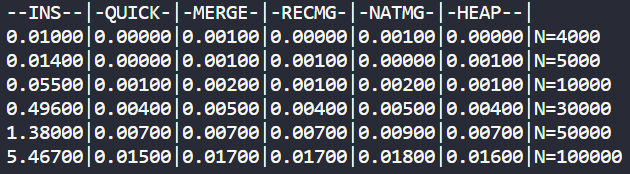
\includegraphics[width=0.5\textwidth]{random_result}}
\subfigure[Graph]{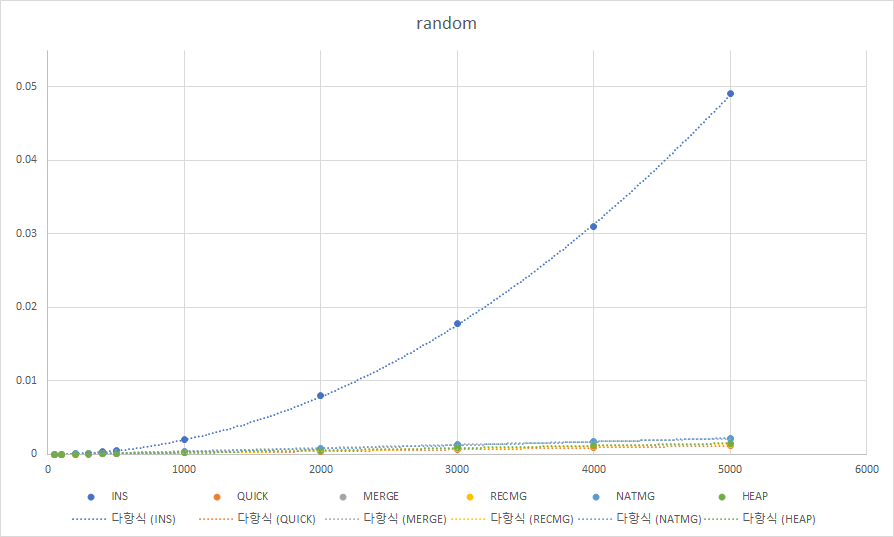
\includegraphics[width=0.5\textwidth]{random_graph}}
\caption{Random.txt}
\label{fig:fig1}

무작위로 나열된 수들이라서 평균성능이 제일 안좋은 삽입정렬(O($n^2$))을 제외하고는 비슷비슷한 성능을 보여주고있다.
\end{figure}
\subsection{partially sorted}
\begin{figure}[h]
\subfigure[Result]{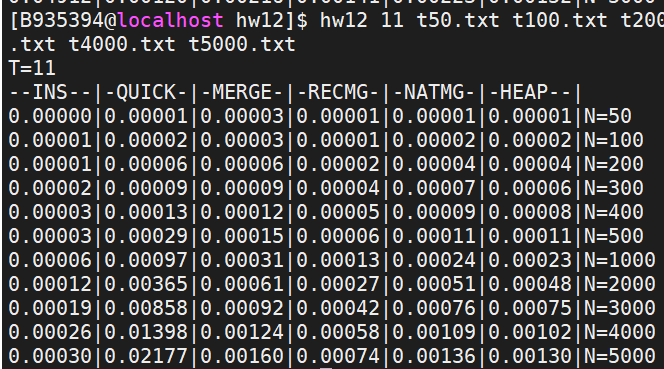
\includegraphics[width=0.5\textwidth]{psorted_result}}
\subfigure[Graph]{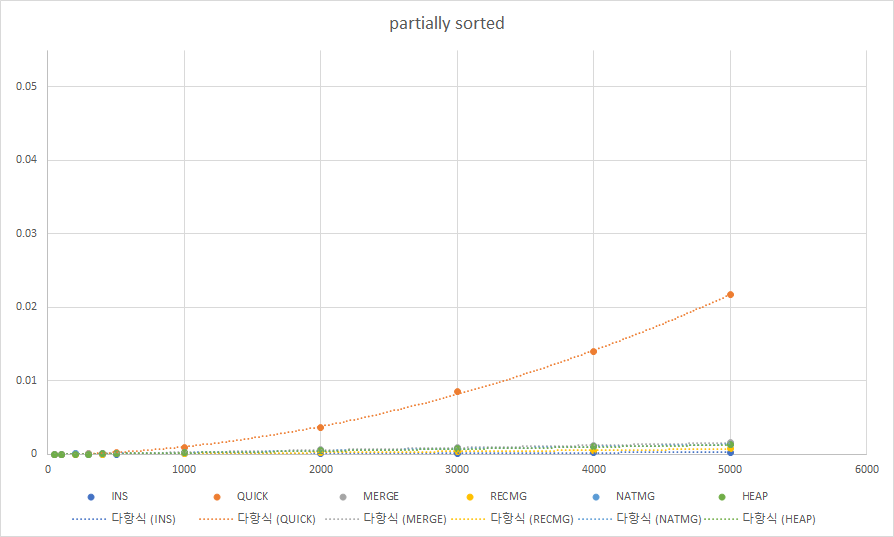
\includegraphics[width=0.5\textwidth]{psorted_graph}}
\caption{PartiallySorted.txt}
\label{fig:fig2}
\end{figure}

배웠던 것처럼 부분적으로 정렬되어있는 리스트에 대해서 삽입함수의 성능이 좋아진 것을 볼 수 있다. 아마 이동 횟수가 적어져서 그런 것 같다. 퀵 정렬의 경우 피벗을 기준으로 양 옆 리스트의 균형이 무너지는 경우가 제법 생겨 성능이 떨어지는 것 같다.
\newpage
\subsection{sorted}
\begin{figure}[h]
\subfigure[Result]{\includegraphics[width=0.5\textwidth]{Sorted_result}}
\subfigure[Graph]{\includegraphics[width=0.5\textwidth]{Sorted_graph}}
\caption{Sorted.txt}
\label{fig:fig3}
\end{figure}

이미 정렬된 수들의 나열이기에 퀵정렬을 제외한 나머지 정렬들은 빠르다. (특히 자연합병정렬) 그러나 퀵 정렬은 피벗 기준 양 옆 리스트의 균형이 무너저 순환 깊이가 평균적으로 기대되는 $\log n$보다 깊어진다. 그래서 6개의 정렬 중 가장 느리다. 

\subsection{decreasing}
\begin{figure}[h]
\subfigure[Result]{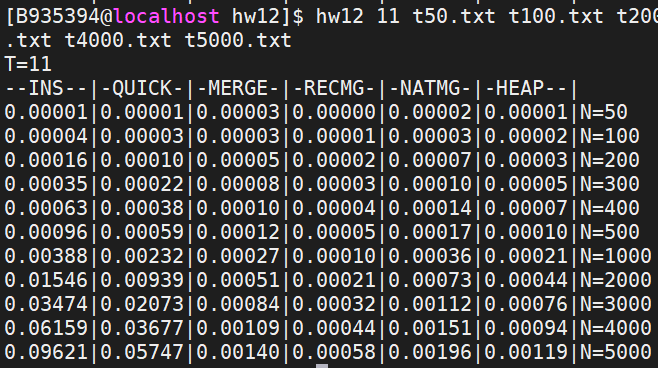
\includegraphics[width=0.5\textwidth]{decreasing_result}}
\subfigure[Graph]{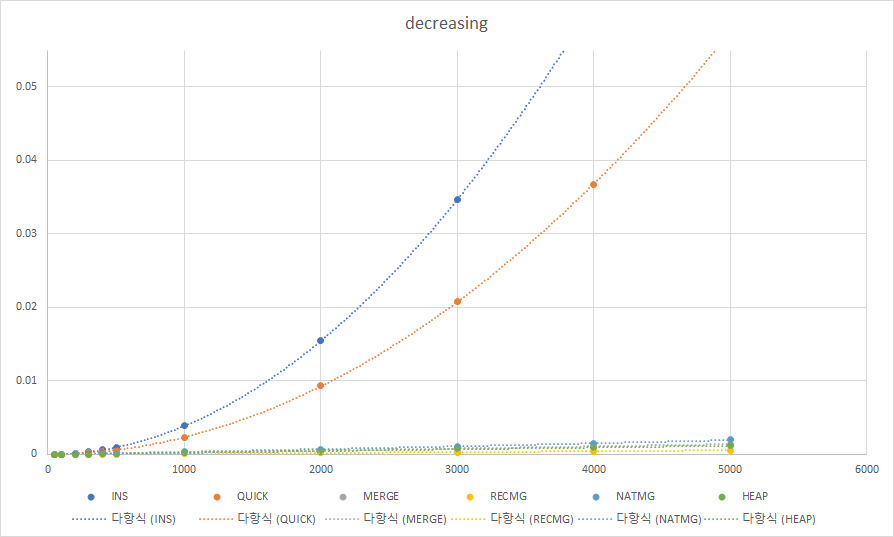
\includegraphics[width=0.5\textwidth]{decreasing_graph}}
\caption{Decreasing.txt}
\label{fig:fig4}
\end{figure}
 
 내림차순으로 정렬된 수들의 나열이다. 자연합병정렬과 반복합병정렬이 사실상 거의 같은 방식으로 돌아가기 때문에 성능이 비슷한 것을 볼 수 있다. 순환합병정렬의 경우 항상 같은 방식을 쓰기 때문에 각 경우(random, partiallysorted....)에서 거의 같은 성능을 보여주는 것을 알 수 있다.(합병하며 정렬해야하는 횟수에 따라 약간의 차이는 존재한다.) 퀵정렬은 양옆리스트 균형이 안맞아 성능이 안좋다. 삽입정렬역시 리스트의 모든 원소를 이동시켜야하기 때문에 성능이 안좋다. \\
 
위의 경우들에서 힙정렬과 3 종류의 합병정렬의 경우에는 특별히 튀는 경우없이 배운 것과 같이 거의 비슷한 성능을 보여주는 것을 알 수 있었다. 퀵정렬 역시 배웠던 대로 리스트의 균형이 무너지는 경우와 평균적인 경우의 성능이 크게 달라졌다. 신기했던 것은 삽입 정렬의 경우였는데, sorted에서 성능이 빠를 것은 짐작하고 있었고 나머지 경우에서 꽤 튀는 성능을 보일 것도 예상했지만, 부분적으로 정렬된 리스트에서 저정도의 성능일 줄은 몰랐었다. 비교횟수의 감소와 이동의 감소가 저정도로 성능에 영향을 줄 수 있다는 점이 신기했다.


\end{document}